\newcommand{\depiction}[1]{\parbox{0.7cm}{\includegraphics[height=0.7cm]{../assets/depictions/#1.pdf}}}
\newcommand{\depictionSM}[1]{\parbox{0.6cm}{\includegraphics[height=0.6cm]{../assets/depictions/#1.pdf}}}


\section{Experiments and results}

Now that the engine, the tools and the methodology are defined, we can proceed to the experiments. Experiments will be divided in three sections: motivation, experiment and results. The motivation will explain why I think the experiment is relevant and present possible hypothesis. The experiment will describe configurations to train different models, how they will be evaluated and what are my expectations. The results will present the data, explain whether my hypothesis was correct or not and give a brief conclusion. \\

Every model's training configuration is defined by the following variables:

\begin{itemize}
\item \textbf{Feature set}: Determinates the encoding of the position, and thus the number of inputs of the model. It conditions which patterns the network can learn. Experimenting with this is the main focus of this thesis.

\item \textbf{Network architecture}: The size of each layer in the network. The first layer (L1) is the feature transformer and it is efficiently updated. The following layer (L2) should be tiny due the NNUE architecture. The size of the model (its complexity) roughly determinates how many patterns the network can learn.

\item \textbf{Dataset}: The positions to train on. The dataset used is explained in detail in chapter 5. In summary, there are 48.5 billion positions to train on and the dataset remains constant across all runs. About 5 million positions are used for validation.

% no me gusta la palabra computed...
\item \textbf{Training method}: Can choose to use either score targets or PQR triplets. This determinates the format of the samples as well as the loss function. All experiments will train using score targets, unless specified. Methods were explained in detail in chapter 5.

\item \textbf{Training hyperparameters}: The usual machine learning hyperparameters for training, such as batch size, learning rate and scheduler. I used the same epoch size used in Stockfish, where each epoch is 100 million positions. Each training run will last for 256 epochs, which means the network is trained in 25.6 billion positions (recall that some of the original 48.5 billion dataset are skipped).
\end{itemize}

Once training is completed, the models will be evaluated depending on the experiment. To assess the performance of a model or to compare a set of models, the following indicators are used:

\begin{itemize}
\item \textbf{Loss}: The training and validation loss are used to detect overfitting and other possible problems. It can't be used to measure the performance of a model. Bigger models must have much better predictions to outweight the cost of having slower inferences and thus less node visits. It's a tradeoff.

\item \textbf{Puzzle accuracy}: The percentage of moves correctly predicted by the engine in Lichess puzzles. Each puzzle may contain multiple moves, and the engine has 100ms per move. Since the engine is not that strong, it does not solve 100\% of puzzles like many other engines do, so I expect differences in this metric to be good indicators. A small set of puzzles is used during training as (a very bad) proxy for the engine's strength, to have early insight of the strength and to detect catastrophic failures that did arise. A bigger set of 85000 puzzles is used after training.

\item \textbf{Relative ELO rating}: A tournament is played between different models to determine their relative strength. Ordo is used to compute the ELO of each model based on the results of the tournament. This is the most important metric, as it is the most reliable way to compare the strength of engines.

% \item \textbf{Inference performance (infs/s)}:

\item \textbf{Training duration}: The amount of time it takes to train a model. This is a one time operation and it does not affect the performance of a model. However, it does condition which and how many experiments I can run.
\end{itemize}

All networks that are not in the first experiment (the baseline), are trained 4 times and a tournament is played between the epoch 192 and 256 of each network (8 networks in total). I have observed a difference of 30 elo points between runs, so this step is crucial to have sensible results. In the appendix are the results of each run and tournament.

\subsection{Baseline}

\textbf{Motivation.} Experiments that will follow will focus on trying out different feature sets, so it is natural to keep every other variable constant. Since the dataset is fixed and the feature set is going to be changing, it remains to find acceptable values for the network architecture and the training hyperparameters. 

Due time and resources constraints, I decided to set the training hyperparameters to   (similar) values which give good results in the official Stockfish trainer: \textbf{a batch size of 16384, a learning rate of 0.0005 and a exponential decay factor of 0.99}. This values showed acceptable results during early stages of development and will remain fixed for all runs.

It remains to find a good network architecture. Bigger networks may have lower loss and predict better, but they will also have slower inferences. This is the tradeoff between inference time and node visits (more depth), which are also affected by the quality of the prediction due to better pruning. So the model must be so much better to compensate the slowdown in inference. \\

\textbf{Experiment.}  In this first experiment I will try different sizes of L1 and L2,  to find an acceptable tradeoff for future experiments. I will run a grid search with L1 $\in \{256, 512, 1024, 2048\}$ and L2 $\in \{32, 64, 128, 256\}$. The feature set used to train will be \featureset{All}, the canonical set with 768 features.

I expect that there will be a model that performs best and other models that are smaller (need stronger predictions) and bigger (need speed to visit more nodes) perform worse. \\

\textbf{Results.} Looking at the result heatmaps in Figure \ref{fig:baseline_heatmaps}, the first thing to notice is that training and validation losses behave as expected. If the model is more complex, meaning the number of parameters (which is dominated by $768*L1+L1*L2$) is higher, the loss is lower and the model predicts better.

When the models are loaded into the engine and evaluated in a tournament, we can see that when L2 drops, the performance drops dramatically. This is due the fact that the inference time is mostly dominated by L2. This result suggests that it may be a good idea explore even lower values of L2, such as 16 or even 8. However, the SIMD implementation requires L2 to be a multiple of 32 so it needs a refactor to keep being fast. So, instead of fiddling further with SIMD I decided to \textbf{keep L2 at 32}.

\begin{figure}[H]
\centering
\makebox[\textwidth]{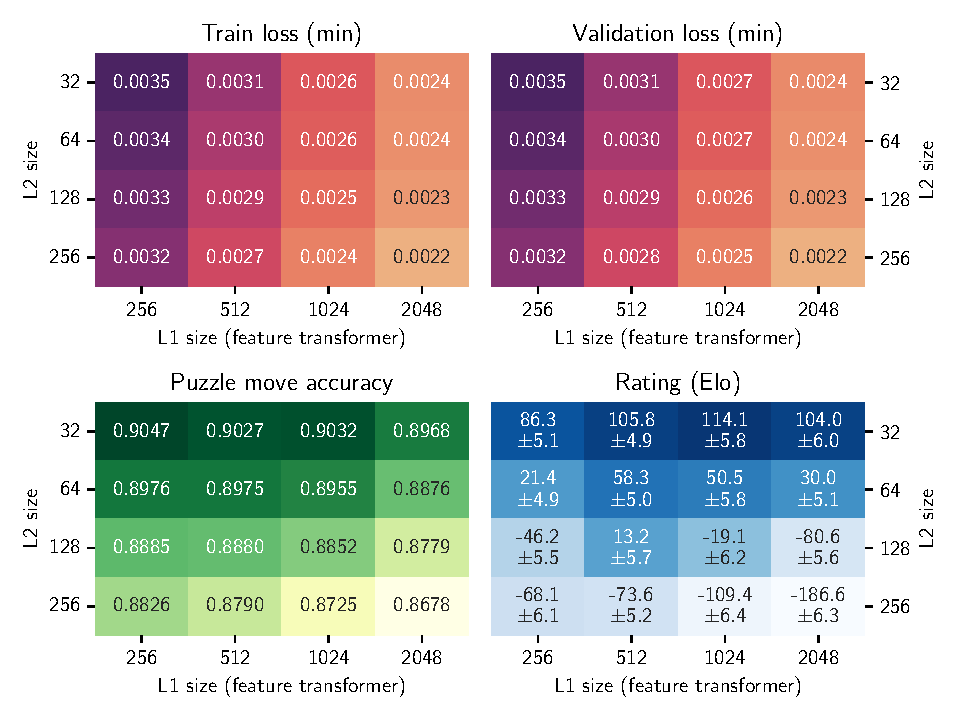
\includegraphics[width=\textwidth]{./dynamic/output/baseline_heatmaps.pdf}}
\captionsetup{justification=centering}
\caption{Network architecture sweep results (L1 $\times$ L2).\\ Table with details in Appendix \ref{appendix:baseline}.}
\label{fig:baseline_heatmaps}
\end{figure}

If L2 is kept constant, the best L1 is not the smallest nor biggest. If L2 $=64$ or L2 $=128$ there is a clear lead of L1 $=512$ in both. In the case of L2 $=32$, the best L1 is not clear because the differences in rating are small and are within margin of error, excluding L1 $=256$ which is definitely wrose. Because training lower values of L1 is faster I opted for \textbf{L1} $\bm{=512}$ due the difference being small and being the best in other L2 values.

So, further experiments will use L1 $=512$ and L2 $=32$. For reference, Stockfish currently uses L1=2560, and employ (lots of) more tricks to make it even faster. The values selected here are specific to the current implementation of the engine, since it may change if more optimizations are made (tradeoff is altered). For this reason, no further modifications to the engine were made after starting with the experiments. We can now proceed with more interesting experiments.

\subsection{Axis encodings}
\label{sec:axis_encoding}

\textbf{Motivation.} Looking back at the networks generated by \featureset{All} in baseline runs, the learned weigths of most neurons in the feature transformer layer (L1) are related with the movement pattern of the pieces. Let's take the example in Figure \ref{fig:rook_weights}, which depicts the \featureset{Square} part of the features where the role is \symrook\ Rook.

\begin{figure}[h]
\centering
\subfloat[\centering $\white$ White]{{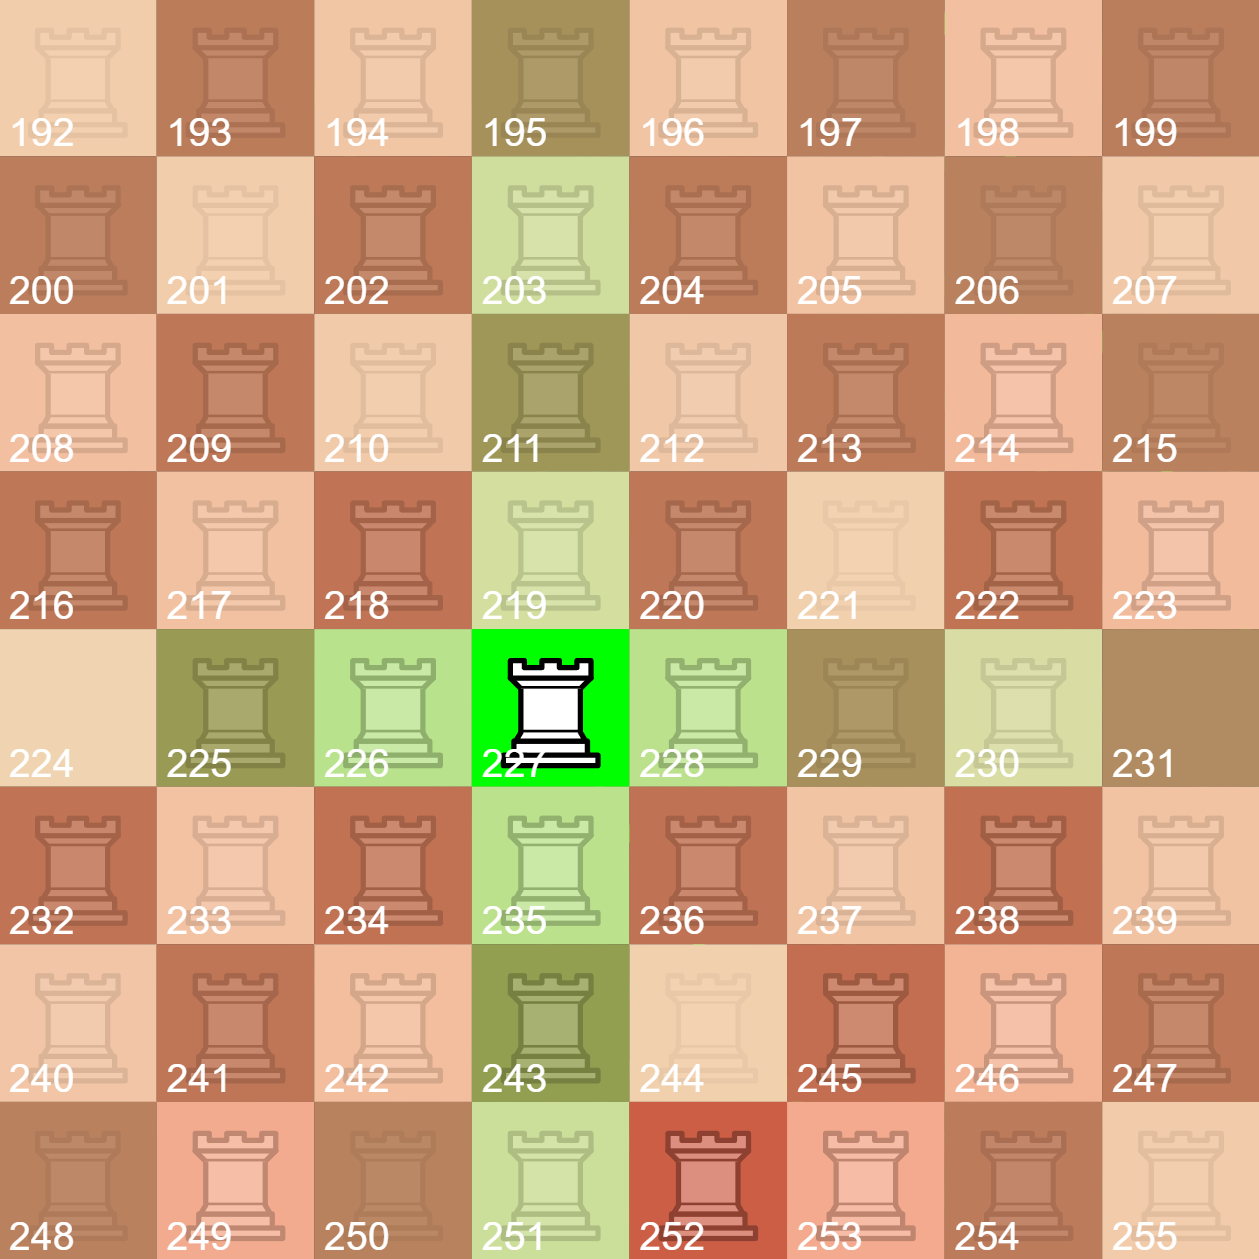
\includegraphics[width=7cm]{../assets/results/piece_weights/white_rook_weights.png} }}%
\qquad
\subfloat[\centering $\black$ Black]{{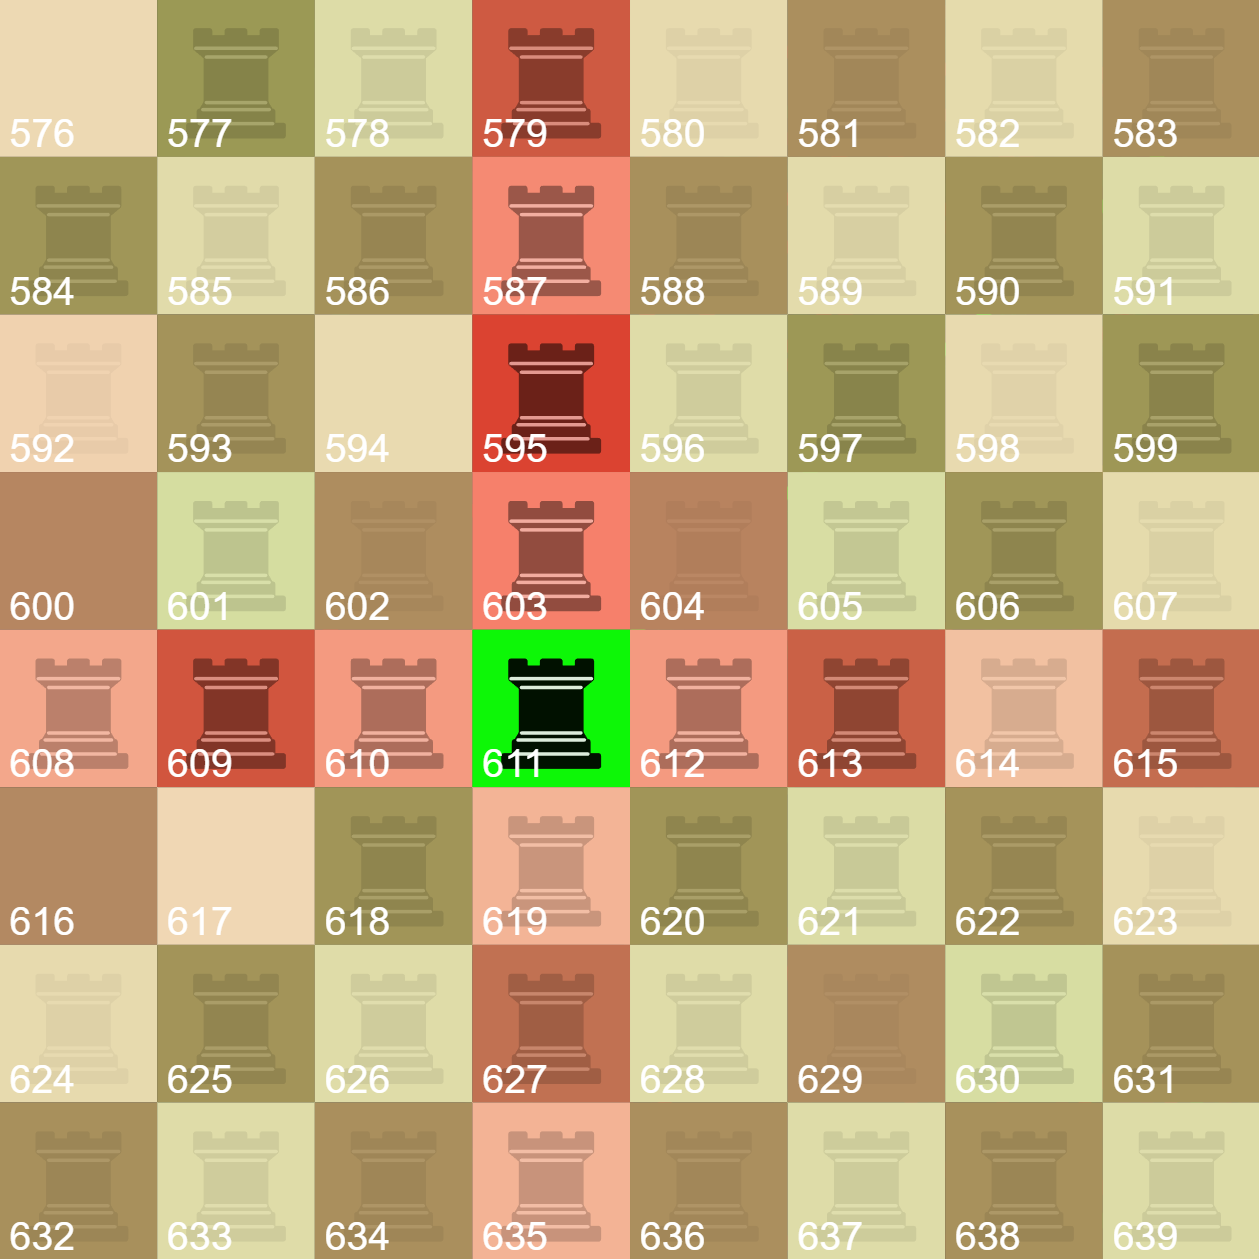
\includegraphics[width=7cm]{../assets/results/piece_weights/black_rook_weights.png} }}%
\caption{Weights of \textbf{a neuron} in the L1 layer, which are connected to features in \featureset{All} where the role is $\rook$ Rook. The intensity represents the weight value, and the color represents the sign (although not relevant).}
\label{fig:rook_weights}
\end{figure}

This particular neuron learned to recognize the presence of a \symrook\ Rook, affected by the pattern of another potential rook in the same file or rank (other pieces may be involved but I am focusing on rooks for the example). Doing so, it had to relate one feature for every potential square where a rook could be for that specific center location, which restrains the network from learning more complex patterns and it is harder to train, because you need more samples to account for all possible combinations.

What if we add a feature which describes \enquote{\textit{there is a $\white$ White $\rook$ Rook in the 4th rank}}? Certainly, this would make the network's job easier, as it would only need to learn the presence of rooks in the corresponding file or rank, instead of every square. This idea can be extrapolated to diagonals, to ease patterns with $\bishop$ Bishops and the $\queen$ Queen.

More examples of this behaviour can be found in Appendix \ref{appendix:axis_samples}, showcasing diagonal patterns and the $\knight$ Knight movements, although they do not move straight through axes. \\

\textbf{Experiment.} I built blocks of features for each natural axis of a chess board, which coincide with the movement pattern of the pieces:

\begin{table}[H]
\centering
\begin{tabular}{cccc}
\depiction{H} & \depiction{V} & \depiction{D1} & \depiction{D2} \\
Horizontal & Vertical & Diagonal 1 & Diagonal 2 \\
(across files) & (across ranks) &  & 
\end{tabular}
\end{table}

% The canonical \featureset{All} feature set encodes each piece's position using the square it is located. Note that this is the same thing as encoding the position for a piece $P$ as $\featureset{File}_{P} \times \featureset{Rank}_{P}$. So the position of each piece is determined using the vertical (across ranks) and horizonal (across files) axes.

In table \ref{tab:axes_blocks} I present the feature blocks. Each block will encode whether there is a piece with the role and color in a specific location along that axis, as explained in the example.

\begin{table}[H]
\caption{Axes feature blocks}
\label{tab:axes_blocks}
\centering

\newcommand{\fullrolecolor}{$\times$ $\featureset{Role}_{P} \times \featureset{Color}_{P}$}

\begin{tabular}{cccccc}
\toprule
\bf Depiction & \bf Block name & \multicolumn{2}{c}{\makecell{\bf Definition\\for every piece $P$ in the board}} & \bf \makecell{Number of\\features} \\
\toprule
\depiction{H} & $\featureset{H}$ & $\featureset{File}_{P}$ & \fullrolecolor & 96 \\
\depiction{V} & $\featureset{V}$ & $\featureset{Rank}_{P}$ & \fullrolecolor & 96 \\
\depiction{D1} & $\featureset{D1}$ & $\featureset{Diag1}_{P}$ & \fullrolecolor & 180 \\
\depiction{D2} & $\featureset{D2}$ & $\featureset{Diag2}_{P}$ & \fullrolecolor & 180 \\
\bottomrule
\end{tabular}

\end{table}


With this blocks, I built different feature sets (listed in table \ref{tab:axis_encoding}): one group of feature sets is just combinations of all the blocks, and another group which is the same as the first but alongside the \featureset{All} feature set (here treated as a block). The second group is the aim of the experiment, it has the classic \featureset{All} feature set but includes the axis blocks to see if the network can benefit from them. The first group, which does not include \featureset{All} is to know how far the network can go only with this blocks alone.

\begin{table}[H]
\caption{Axis encodings feature sets}
\label{tab:axis_encoding}
\centering

\newcommand{\rolecolor}{$\times$ $\featureset{R}_{P} \times \featureset{C}_{P}$}

\begin{tabular}{ccc}
\toprule
\bf Depiction & \bf Feature set & \bf \makecell{Number of\\features} \\
\toprule
\depiction{H} $\oplus$ \depiction{V} & $\featureset{H} \oplus \featureset{V}$ & 192 \\
\midrule
\depiction{D1} $\oplus$ \depiction{D2} & $\featureset{D1} \oplus \featureset{D2}$ & 360 \\
\midrule
\depiction{H} $\oplus$ \depiction{V} $\oplus$ \depiction{D1} $\oplus$ \depiction{D2} & $\featureset{H} \oplus \featureset{V}$ $\oplus$ $\featureset{D1} \oplus \featureset{D2}$ & 552 \\
\midrule
% ------------------------------------
\midrule
\featureset{All} $\oplus$ \depiction{H} $\oplus$ \depiction{V} & $\featureset{All} \oplus \featureset{H} \oplus \featureset{V}$ & 960 \\
\midrule
\featureset{All} $\oplus$ \depiction{D1} $\oplus$ \depiction{D2} & $\featureset{All} \oplus \featureset{D1} \oplus \featureset{D2}$ & 1128 \\
\midrule
\featureset{All} $\oplus$ \depiction{H} $\oplus$ \depiction{V} $\oplus$ \depiction{D1} $\oplus$ \depiction{D2} & \featureset{All} $\oplus$ \featureset{H} $\oplus$ \featureset{V} $\oplus$ \featureset{D1} $\oplus$ \featureset{D2} & 1320 \\
\bottomrule

\end{tabular}
\end{table}

I expect that the feature sets that are sums of single axes ($\depictionSM{H} \oplus \depictionSM{V}, \depictionSM{D1} \oplus \depictionSM{D2}$ and $\depictionSM{H} \oplus \depictionSM{V} \oplus \depictionSM{D1} \oplus \depictionSM{D2}$) will perform worse overall, since to capture the exact position of pieces in the board, the network will have to learn to relate at least two features for every location. This information is already available when \featureset{All} is present.

The feature sets that include \featureset{All} (\featureset{All} $\oplus \hdots$) should perform better than without, providing that the idea explained in the motivation holds.

For each of the proposed feature sets, I will train a network and evaluate its performance relative to each other using a tournament. I expect to see them ranked in the reverse order as presented in the table (more extra axes better). \\

\textbf{Results.} The results in table \ref{tab:axis_results} show that indeed, adding the axes blocks make the network validation loss slightly lower, from 0.00316 in \featureset{All} to 0.00307 including all four blocks. However, this improvement in loss is not significant enough to make the network stronger to compensate the (small) performance hit of having more features. As you can see in the table, including more axes makes the loss decrease slightly yet the rating decreases by a huge factor.

All three feature sets that do not include \featureset{All} unsuprisingly perform much, much worse even having less features. The feature set \featureset{H+V+D1+D2} has a 25\% higher loss than \featureset{All} and $172.5 \pm 4.8$ less rating than \featureset{All}. The other feature sets in this group perform even worse, as it was expected.

I discovered that the accuracy of puzzles is not a good a proxy of an engine's strength, given that there is a 474 rating difference yet 3\% a difference in move accuracy. I believe that the reason lies on the fact that puzzles may be more strategic than positional. I will drop the puzzle accuracy metric in future experiments.

\begin{table}[H]
\caption{Axis encodings results}
\label{tab:axis_results}
\centering

% 1 256-eval_16384_(hv[768]→512)x2→32→1.nn          :     0.0   ----  22665.5   32456    70      96
% 2 256-eval_16384_(hv+h+v[960]→512)x2→32→1.nn      :    -4.6    5.0  22474.0   32456    69     100
% 3 256-eval_16384_(hv+d1+d2[1128]→512)x2→32→1.nn   :   -33.3    5.0  21260.5   32456    66     100
% 4 256-eval_16384_(hv+h+v+d1+d2[1320]→512)x2→32→1.nn   :   -57.7    4.8  20207.5   32458    62     100
% 5 256-eval_16384_(h+v+d1+d2[552]→512)x2→32→1.nn   :  -172.5    4.8  15176.0   32456    47     100
% 6 256-eval_16384_(h+v[192]→512)x2→32→1.nn         :  -368.1    5.7   7527.0   32460    23     100
% 7 256-eval_16384_(d1+d2[360]→512)x2→32→1.nn       :  -474.5    6.4   4289.5   32458    13     ---

% Network: 256-eval_16384_(d1+d2[360]→512)x2→32→1.nn Accuracy: 0.851789055191768
% Network: 256-eval_16384_(h+v+d1+d2[552]→512)x2→32→1.nn Accuracy: 0.8748684518241348
% Network: 256-eval_16384_(h+v[192]→512)x2→32→1.nn Accuracy: 0.8618817235734331
% Network: 256-eval_16384_(hv+d1+d2[1128]→512)x2→32→1.nn Accuracy: 0.8814458606173995
% Network: 256-eval_16384_(hv+h+v+d1+d2[1320]→512)x2→32→1.nn Accuracy: 0.8766955098222639
% Network: 256-eval_16384_(hv[768]→512)x2→32→1.nn Accuracy: 0.8865762394761459
% Network: 256-eval_16384_(hv+h+v[960]→512)x2→32→1.nn Accuracy: 0.8851511342376053

\begin{tabular}{cccccc}
\toprule
\bf Feature set  & \bf \makecell{Number\\of features} & \makecell{\bf Val. loss\\\textit{min}} & \makecell{\bf Rating\\\textit{elo (rel. to \featureset{All})}} & \makecell{\bf Puzzles\\\textit{move acc.}} \\
\toprule
\depiction{H} $\oplus$ \depiction{V} & 192 & 0.00581 & -368.1 $\pm$ 5.7 & 0.8618 \\
\midrule
\depiction{D1} $\oplus$ \depiction{D2} & 360 & 0.00670 & -474.5 $\pm$ 6.4 & 0.8517 \\
\midrule
\makecell{\depiction{H} $\oplus$ \depiction{V} $\oplus$ \\ \depiction{D1} $\oplus$ \depiction{D2}} & 552 & 0.00389 & -172.5 $\pm$ 4.8 & 0.8748 \\
\midrule
% ------------------------------------
\midrule
\featureset{All} (reference) & 768 & 0.00316 & \textbf{0.0} & 0.8865 \\
\midrule
\featureset{All} $\oplus$ \depiction{H} $\oplus$ \depiction{V} & 960 & 0.00308 & -4.6 $\pm$ 5.0 & 0.8851 \\
\midrule
\featureset{All} $\oplus$ \depiction{D1} $\oplus$ \depiction{D2} & 1128 & 0.00309 & -33.3 $\pm$ 5.0 & 0.8814 \\
\midrule
\makecell{\featureset{All} $\oplus$ \depiction{H} $\oplus$ \depiction{V} \\ \hspace{0.75cm} $\oplus$ \depiction{D1} $\oplus$ \depiction{D2}} & 1320 & \textbf{0.00307} & -57.7 $\pm$ 4.8 & 0.8766 \\
\bottomrule

\end{tabular}
\end{table}

The next experiment will focus on adding more specific features, instead of more broad ones.


\subsection{Pairwise axes}

Pepito \depiction{PH} asdo \depiction{PV} asd\depiction{PD1} asd\depiction{PD2} asd

[explicar...]

3 runs
HV + PH
HV + PV
HV + PH + PV

el cosito de los pares \\

los resultados no son buenos...

I did not bother implementing diagonal pairs.


\noindent\rule{\textwidth}{1pt}

\vspace{0.2cm}
Up to this point, I have been trying to encode the position of the pieces in different or smarter ways, with no avail. It may seem that the network is able to extract all the information it needs from the most basic \featureset{All} feature set. Making the information available in another form makes no difference, as opposed to what I originally thought.

Further experiments will focus on features not related to the position of the pieces, but to other aspects of the game, inspired by hand crafted evaluations.

\noindent\rule{\textwidth}{1pt}


\subsection{Mobility}

\textbf{Motivation.} Mobility in chess is a measure of the available moves a player can make in a given position. The idea is that if a player has more available moves, the position is stronger. In \cite{slater:1950} it was shown that there is a strong correlation between a player's mobility and the number of games won. This metric has been used extensively in hand crafted evaluations, and I propose to include this information as features for the neural network.

There are a couple of ways to go about encoding mobility:

\begin{itemize}
\item \textbf{Bitsets (per piece type):} the amount of features changed each turn may negate any gains.

\begin{figure}[h]
\centering

\begin{tabular}{ccccc}

\raisebox{-7ex}{\chessboard[
    setfen=r5k1/1b1p1ppp/p7/1p1Q4/2p1r3/PP4Pq/BBP2b1P/R4R1K w - - 0 20,
    tinyboard,
    showmover=false,
]}
&

\raisebox{-7ex}{\chessboard[
    tinyboard,
    showmover=false,
    setwhite={ba2,bb2},
    pgfstyle=color,
    opacity=0.8,
    color=blue,
    markfield={b1,c1,c3,d4,e5,f6,g7}
]}

&

\raisebox{-7ex}{\chessboard[
    tinyboard,
    showmover=false,
    addblack={Bb7,Bf2},
    pgfstyle=color,
    opacity=0.8,
    color=blue,
    markfield={c8,c6,d5,a7,b6,c5,d4,e3,e1,g1,g3}
]}

&

\raisebox{-7ex}{\chessboard[
    tinyboard,
    showmover=false,
    setwhite={qd5},
    pgfstyle=color,
    opacity=0.8,
    color=blue,
    markfield={d6,d7,e6,f7,e5,f5,g5,h5,e4,d4,d3,d2,d1,c4,c5,b5,c6,b7}
]}

& $\hdots$

\\

Board &
\makecell{\white White\\\symbishop\ Bishop} &
\makecell{\black Black\\\symbishop\ Bishop} &
\makecell{\white White\\\symqueen\ Queen}

\end{tabular}
\end{figure}


\item \textbf{Counts (per piece type):}
\end{itemize}


\newpage
\subsection{PQR}

\textbf{Motivation.} During the initial research for a thesis subject, I came across \cite{dlchess:2014} which seemed an interesting approach to train a neural network to evaluate positions. Since it was released in 2014, it predates the NNUE era and the training data was suboptimal (Lichess database \cite{lichessdb} with human moves). So I decided to try to replicate the idea using modern datasets, better moves and a proper engine. The \enquote{PQR} method itself was explained in detail in the previous chapter.  Remember that $p$ is a position in the dataset, $q$ is the position obtained by making the best move according to the dataset and $r$ is a random position obtained making a random move from $p$ such that $r \neq q$. \\

Before starting the experiment, I checked if existing networks trained with the conventional method behave under the principles of the PQR method: ${f(p) = -f(q)}$ and ${f(r) > f(q)}$. In the left plot of figure \ref{pqr-eval}, we can see that values of $f(p)$ and $f(q)$ are negatively correlated, which supports the principle that $f(p)=-f(q)$. In the right plot, we can see that the distribution of the difference between $f(r)$ and $f(q)$ is mostly positive, which supports the principle that $f(r) > f(q)$. This shows that the principles that the PQR method relies on are properties that manifest in existing models.

\begin{figure}[H]
\centering
\makebox[\textwidth]{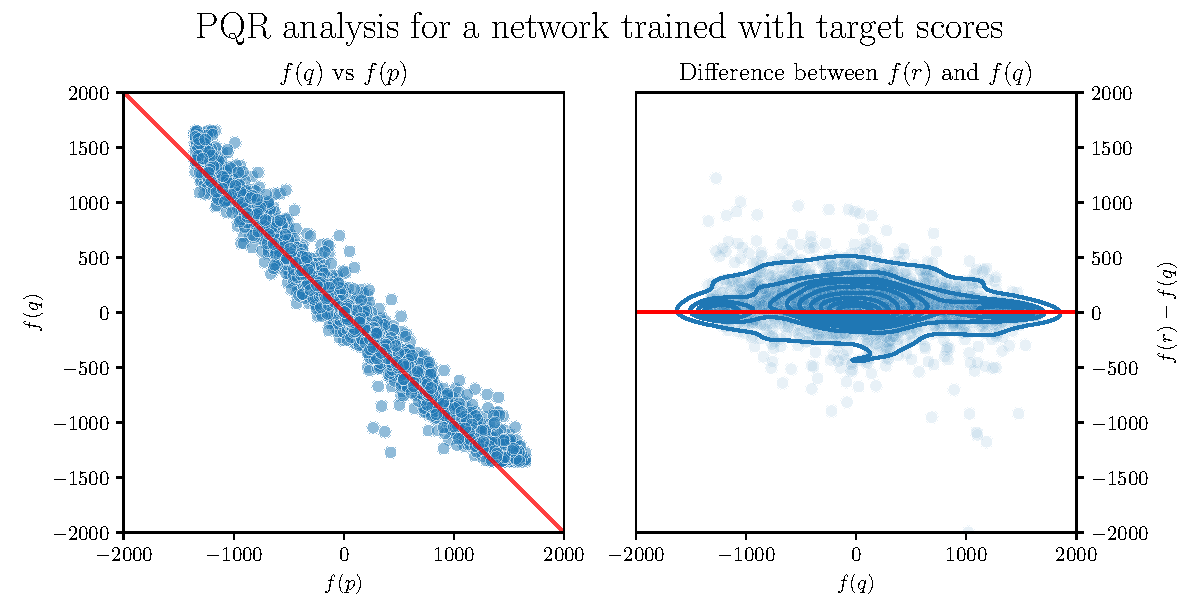
\includegraphics[width=\textwidth]{../dynamic/output/pqr_eval.pdf}}
\caption{Analysis of $N=10000$ PQR positions using a model trained with target scores and the feature set \featureset{All}.}
\label{pqr-eval}
\end{figure}

\textbf{Experiment.} I will train the canonical \featureset{All} feature set with this method in two ways:

\begin{itemize}
\item \textbf{Train from scratch.} The network is initialized with random weights and trained with the PQR method. This is what the original authors did, and I do not expect to reach the performance of models trained with the evaluations method. Using precomputed evaluations as a target is a lot simpler for the model, since it only has to learn to mimic the scores.

\item \textbf{Train from a checkpoint.} A strong checkpoint trained with the other method is used to initialize the network. This way, the network does not have to learn too much at once and may enable it to improve the existing parameters. I believe that two scenarios are likely to happen: the model improves very slowly, or it completely forgets what it have learned before and ends up like a model trained from scratch. The best scenario is that the model improves slowly, proving that it can be used to further optimize existing models.
\end{itemize}

\textbf{Results.}


aqui pondria los resultados... si los tuviera!


%\subsection{Active neurons}
%medir si hay feature sets que no usen neuronas, que esto disparo el uso de HalfTopK
%average number of features enabled by feature set (cantidad y porcentaje)
%measure updates per move average and refreshes average per FS
%[ESTO PONERLO EN EL APPENDIX]


%%%%%%%%%%%%%%%%%%%%%%%%%%%%%%%%%%%%%%%%%%%
%%%%%%%%%%%%%%%%%%%%%%%%%%%%%%%%%%%%%%%%%%%
%%%%%%%%%%%%%%%%%%%%%%%%%%%%%%%%%%%%%%%%%%%
%%%%%%%%%%%%%%%%%%%%%%%%%%%%%%%%%%%%%%%%%%%
%%%%%%%%%%%%%%%%%%%%%%%%%%%%%%%%%%%%%%%%%%%
%%%%%%%%%%%%%%%%%%%%%%%%%%%%%%%%%%%%%%%%%%%
%%%%%%%%%%%%%%%%%%%%%%%%%%%%%%%%%%%%%%%%%%%
%%%%%%%%%%%%%%%%%%%%%%%%%%%%%%%%%%%%%%%%%%%
%%%%%%%%%%%%%%%%%%%%%%%%%%%%%%%%%%%%%%%%%%%
%%%%%%%%%%%%%%%%%%%%%%%%%%%%%%%%%%%%%%%%%%%
%%%%%%%%%%%%%%%%%%%%%%%%%%%%%%%%%%%%%%%%%%%



\subsection{Attacks / Threats}

as bitsets per piece type
number of attacks

\subsection{mas supongo?}

\subsection{Symmetry? / Relativity?}

\textbf{Motivation.}

BUCKETING

Medir el impacto de agregar simetría al fs. Red mas chica, inf mas rapida, mejor perf?

probar simetria, eventualmente probar con el mejor feature set de arriba, a ver si mejora poniendo a cada bloque individual simetria

\featureset{Half-Relative(H|V|HV)King-Piece}?

inspired by KP, build features relative to the position of the $\king$ King

\subsection{Statistical features?}

Define \featureset{k-All-All}

\featureset{King-All} is a subset of \featureset{All-All}.

Top P

Hacer un subset de \featureset{AA} (589824).

\begin{itemize}
\item Destilar?
\item Probar si es lo mismo quedarse con el TOP K de las mas comunes o con las que dice el performance.
\item Catboost? PCA?
\end{itemize}
